% Use only LaTeX2e, calling the article.cls class and 12-point type.

\documentclass[11pt]{article}
\usepackage[round,semicolon]{natbib}
\usepackage[margin=1.25in]{geometry}
\usepackage{kpfonts}

\usepackage{seqsplit}
\usepackage{placeins}

\usepackage{newfloat}
\usepackage[labelfont=bf]{caption}
\usepackage{nameref}
\usepackage{rotating}
\usepackage{color}
\usepackage{float}

\setcounter{topnumber}{8}
\setcounter{bottomnumber}{8}
\setcounter{totalnumber}{8}
\renewcommand{\topfraction}{1}
\renewcommand{\bottomfraction}{1}
\renewcommand{\textfraction}{0}
\renewcommand{\floatpagefraction}{1}

\usepackage[font=small,labelfont=bf]{caption}

\usepackage{newfloat}
\DeclareFloatingEnvironment[name={Figure}]{suppfigure}
\renewcommand{\thesuppfigure}{S\arabic{suppfigure}}
\DeclareFloatingEnvironment[name={Table}]{supptable}
\renewcommand{\thesupptable}{S\arabic{supptable}}
\DeclareFloatingEnvironment[name={File}]{suppfile}
\renewcommand{\thesuppfile}{S\arabic{suppfile}}

\definecolor{darkblue}{rgb}{0, 0.0, 0.6}

\usepackage{hyperref}
\hypersetup{colorlinks,citecolor=blue,linkcolor=blue,urlcolor=blue}

\usepackage{seqsplit}

\usepackage{array}
\newcolumntype{R}[1]{>{\raggedright\arraybackslash}p{#1}}
\newcolumntype{C}[1]{>{\centering\let\newline\\\arraybackslash\hspace{0pt}}m{#1}}

\newcommand{\comment}[1]{{\color{red}[\textsl{#1}]}}

\usepackage{setspace}

\renewcommand{\topfraction}{1}
\renewcommand{\bottomfraction}{1}
\renewcommand{\textfraction}{0}
\renewcommand{\floatpagefraction}{1}


\title{Deep mutational scanning of an H3 hemagglutinin can inform evolutionary forecasting of human H3N2 influenza virus} 

\author{
Juhye M. Lee$^{1,4,5,\dagger}$ \and 
John Huddleston$^{2,6,\dagger}$ \and 
Michael B. Doud$^{1,4,5}$ \and 
Kathryn A. Hooper$^{1,6}$ \and
Trevor Bedford,$^{2,3}$ \and 
Jesse D. Bloom$^{1,3,4*}$
\\
\scriptsize{$^1$Basic Sciences Division, $^2$Vaccine and Infectious Diseases Division, and $^3$Computational Biology Program,} \\
\scriptsize{Fred Hutchinson Cancer Research Center, Seattle, WA, USA} \\
\scriptsize{$^4$Department of Genome Sciences, $^5$Medical Scientist Training Program, and $^6$Molecular and Cellular Biology Program,} \\
\scriptsize{University of Washington, Seattle, WA, USA} \\
\scriptsize{$^{\dagger}$These authors contributed equally} \\
\scriptsize{$^*$Correspondence: \href{jbloom@fredhutch.org}{jbloom@fredhutch.org}}
}

\date{}


\begin{document}

\maketitle
\onehalfspacing

\begin{abstract}
Abstract text.
\end{abstract}

\section*{INTRODUCTION}

\section*{RESULTS}
\label{sec:results}

\subsection*{Strategy for deep mutational scanning of an H3 hemagglutinin}
Previously, we measured the effect of all possible single amino-acid mutations to a highly lab-adapted H1 hemagglutinin from the A/WSN/1933 (H1N1) strain~\citep{thyagarajan2014inherent,doud2016accurate}. 
To better understand the effects of mutations to a hemagglutinin of more direct relevance to influenza strains currently circulating in the human population, we chose to study H3 HA from the A/Perth/16/2009 (H3N2) strain. 
This strain was the H3N2 component of the influenza vaccine from 2010-2012.
\comment{mention serial passages and TC-adaptation mutations...}

We mutagenized the Perth/2009 HA gene to create mutant plasmid HA libraries encompassing all 567 codons and harboring an average of $\sim$1.4 codon mutations per clone.
We then used a helper-virus system previously established in~\cite{doud2016accurate} to bypass the bottlenecks associated with reverse genetics to generate complex mutant virus libraries from the mutant plasmids (Figure~\ref{fig:dms_overview}A).
In order to maximize viral titers and further avoid bottlenecking the diversity of the initially generated mutant viruses, we used an HA-deficient helper virus carrying WSN/1933 internal and NA genes to rescue the mutant viruses, thereby pairing the mutant HA's with the WSN NA.
Additionally, we used MDCK-SIAT1 cells constitutively expressing the TMPRSS2 protease, which is found endogenously in the human airway and facilitates HA cleavage and activation \comment{cite B\"{o}ttcher 2006 JVI, B\"{o}ttcher-Friebertsh\"{a}user 2010 JVI}.
All of the experiments were completed in full biological triplicate (Figure~\ref{fig:dms_overview}B). 
We also passaged and deep sequenced library 3 in technical replicate (denoted as library 3-1 and 3-2) to gauge to the amount of experimental noise occurring \textit{within} a single biological replicate.

Figure~\ref{fig:dms_overview}C shows the mutation frequencies of the mutant plasmids, mutant viruses, wildtype plasmids and wildtype viruses determined from deep sequencing. 
There is selection against non-functional HA variants as revealed by the reduced mutation frequencies of the mutant viruses compared to their starting frequencies in the mutant plasmids.
Specifically, stop codons were purged to 20-45\% of their original starting frequencies, after correcting for error rates from the wildtype controls.
Although the majority of stop codons were purged, incomplete purging of stop codons is likely due to complementation of defective viral particles by infectious virions. 
We also observed purging of most nonsynonymous mutations to 30-40\% of their initial starting frequencies after error correction, suggesting strong selection against deleterious HA variants.

We next quantified the reproducibility of our deep mutational scanning measurements across biological and technical replicates. 
We inferred the amino-acid preferences at each site in the Perth/2009 HA using the method described in~\cite{bloom2015software} and implemented in the \texttt{dms\_tools2} software [\url{https://jbloomlab.github.io/dms_tools2/}].
These preferences represent an estimate of the 567 sites $\times$ 20 amino acids $=$ 11340 experimental measurements and are normalized to sum to one at each site.
The correlations of the amino-acid preferences between each pair of replicates is shown in Figure~\ref{fig:dms_overview}D.
The biological replicates are fairly well-correlated, with a Pearson's $R$ ranging from 0.69 to 0.78. 
Replicate 1 exhibits the least amount of correlation with the other biological replicates, consistent with the observation that this replicate showed the weakest selection against stop and nonsynonymous mutations and might therefore be subject to more experimental noise.
Of note, the two technical replicates 3-1 and 3-2 were only slightly more reproducible than that between biological replicates.
This suggests that bottlenecking of the virus library during the low MOI passage contributes to much of the noise observed in our experiments, as we are only able to passage a finite number of viral particles.

\begin{figure}
\centerline{\includegraphics[width=\textwidth]{figs/dms_overview/dms_overview.pdf}}
\caption{\label{fig:dms_overview}
{\bf Overview of deep mutational scanning experiments of H3 hemagglutinin.}
(A) We used a helper virus approach previously described in Doud (2016) to generate the mutant virus libraries. 
We transfected MDCK-SIAT1-TMPRSS2 cells with the mutant plasmid library carrying all possible amino-acid mutations to the A/Perth/16/2009 (H3N2) HA, in addition to protein expression plasmids encoding the viral ribonucleoprotein complex. 
After transfection, we infected the cells with an HA-deficient helper virus carrying all of the WSN/1933 (H1N1) influenza genes. 
We then passaged the initially generated pool of mutant viruses at low MOI to establish a genotype-phenotype linkage and select for functional HA variants. 
(B) All of the experiments were completed in biological triplicate, starting from independent preps of the wildtype HA genes to create the mutant plasmids. 
In addition, we passaged and deep sequenced library 3 in technical replicate, denoted 3-1 and 3-2, to estimate the amount of experimental noise within a single biological replicate.
(C) Mutation frequencies of nonsynonymous, stop, and synonymous mutations for the mutant DNA, mutant virus, wildtype DNA, and wildtype virus samples. 
There is selection against nonsynonymous and stop codons in the mutant viruses. 
The percentages signify the frequency of stop codons remaining in the passaged mutant viruses relative to their starting frequency in the mutant plasmid libraries after correcting for the stop codon frequencies in the wildtype DNA and viruses.
(D) The correlations and the Pearson correlation coefficient for the amino-acid preferences between each pair of replicates are shown. 
The biological replicates are fairly well-correlated, as are the technical replicates, indicating some degree of bottlenecking of variants during the viral passage which can contribute to experimental noise. 
}
\end{figure}


\subsection*{H3 site-specific amino-acid preferences}
How well do the Perth/2009 HA preferences inferred from experimental measurements describe the evolution of H3N2 influenza virus in nature?
\comment{phydms analysis here}

\begin{figure}
\centerline{\includegraphics[width=\textwidth]{figs/mut_tolerance/entropy_heatmap.pdf}}
\caption{\label{fig:mut_tolerance}
{\bf Different regions of HA exhibit varying degrees of mutational tolerance.}
Mutational tolerance as calculated by the Shannon entropy of a given site's amino-acid preferences are mapped onto the structure of the H3 trimer (PDB 4O5N, \comment{cite}) and the H1 trimer (PDB 1RVX, \comment{cite}), with both trimers in approximately the same orientation. 
The site entropies were calculated from the preferences measured in the Perth/2009 H3 (left panel) or the preferences measured in the WSN/1933 H1 (right panel). 
Lighter shades of blue or red signify low mutational tolerance, while darker shades of blue or red signify high mutational tolerance. 
For each HA, the structure on the left side colors the full HA trimer, while the structure on the right side colors only one of the monomers.
The sialic acid receptor is shown as black sticks.
The Perth/2009 H3 shows relatively high mutational tolerance in the stalk region compared to the head region. 
The head region of the WSN/1933 H1 is mutationally tolerant compared to the relatively intolerant stalk region. 
}
\end{figure}

\begin{figure}
\centerline{\includegraphics[width=\textwidth]{figs/prefslogoplot/rescaled-avgprefs_prefs.pdf}}
\caption{\label{fig:logoplot}
{\bf The site-specific amino-acid preferences of H3 hemagglutinin.}
This logoplot shows the site-specific amino-acid preferences for the averaged replicates rescaled by the stringency parameter (Table 1) estimated by phydms.
The height of each letter is proportional to its preference at that site, and the preferences for all sites are normalized to sum to 1.
The sites are in H3 numbering.
The top overlay bar shows the relative solvent accessibility.
The bottom overlay bar is colored by the HA domain (sig. pep. = signal peptide, HA1 ecto. = HA1 ectodomain, HA2 ecto. = HA2 ectodomain, TM = transmembrane domain, cyto. tail. = cytoplasmic tail).
The letters directly above each logo indicate the wildtype amino acid at that site.
}
\end{figure}


\subsection*{Estimating mutational effects from an H3N2 phylogeny}

\begin{figure}
\centerline{\includegraphics[width=\textwidth]{figs/trunkvssidebranch/trunkvssidebranch.pdf}}
\caption{\label{fig:trunkvssidebranch}
{\bf The trunk of a human H3N2 phylogeny has higher mutational effects than those of side branches.}
(A) Phylogenetic tree of human H3N2 influenza virus from 1968-present. 
\comment{We downloaded X sequences from the Influenza Virus Resource ?.... etc. inferred the tree, ancestral state reconstruction, visualized the tree. Mark Perth/2009 on the tree}
To parse out trunk mutations from side branch mutations, we first defined a set of recent nodes sampled on or after Jan. 1, 2017, and traced these nodes back to their most recent common ancestor. 
All branches ancestral to the MRCA of the recent nodes were defined as the trunk (shown in red), and all other branches were defined as side branches (shown in blue).
(B) Using the Perth/2009 H3 preferences, we calculated the log$_{2}$ mutational effect for trunk and side branch mutations in windows of 5 years for every year from 1968-2013. 
The median log$_{2}$ mutational effect in a given window is shown as circles for trunk mutations and triangles for side branch mutations. 
The shaded region demarcates the interquartile range of trunk and side branch mutational effects.
The median trunk mutational effects are consistently higher than the median side branch mutational effects for all windows.
(C) The log$_{2}$ mutational effect for all side branch and all trunk mutations (left panel), in addition to all mutations in internal nodes and terminal nodes on the side branches (right panel) are shown.
To estimate significance, we performed 10,000 randomizations of the preferences to calculate the median difference in trunk vs side branch mutational effects, and counted how many of the randomizations exceeded the true difference in median trunk vs side branch mutational effects.
The effects of trunk mutations are higher than side branch, internal and terminal node, mutations.
}
\end{figure}

\begin{figure}
\centerline{\includegraphics[width=\textwidth]{figs/sequence_preference/sequence_preference.pdf}}
\caption{\label{fig:sequence_preference}
{\bf The trunk exhibits higher sequence preference than side branches.}
figure text
}
\end{figure}

\begin{figure}
\centerline{\includegraphics[width=\textwidth]{figs/WSN_trunkvssidebranch/WSN_trunkvssidebranch.pdf}}
\caption{\label{fig:WSN_trunkvssidebranch}
{\bf The WSN/1933 H1 preferences do not reveal differences in trunk vs side branch mutational effects}
(A) We calculated the log$_{2}$ mutational effects of the same set of trunk and side branch mutations from the inferred H3N2 phylogeny in Figure~\ref{fig:trunkvssidebranch} using the WSN/1933 H1 preferences.
We again randomized the preferences for a total of 10,000 iterations and counted the number of randomizations that exceeded that true difference in median trunk vs side branch mutational effects to calculate a p-value.
Using the WSN/1933 H1 preferences, there is not a significant difference in trunk vs side branch mutational effects.
(B) We also performed the same sliding window analysis shown in Figure~\ref{fig:muteffects_sliding_window}, but using the WSN/1933 H1 preferences.
There is not a distinct difference in trunk and side branch mutational effects.
}
\end{figure}


\subsection*{Comparing H1 and H3 preferences}

\begin{figure}
\centerline{\includegraphics[width=\textwidth]{figs/distance_distribution/distance_distribution.pdf}}
\caption{\label{fig:distance_distribution}
{\bf The HA homologs exhibit many large shifts in preference compared to shifts for other viral protein homologs}
(A) A phylogenetic tree of the HA subtypes, with the two HA's, WSN/1933 H1 and Perth/2009 H3, for which we have measured amino-acid preferences denoted on the tree. 
The WSN/1933 H1 and the Perth/2009 H3 share $\sim$42\% amino-acid identity.
(B) The correlation for the amino-acid preferences for replicates both within and between the two HA homologs.
(C) The distribution of shifts in preference for various homolog pairs are shown.
}
\end{figure}

\begin{figure}
\centerline{\includegraphics[width=\textwidth]{figs/RMSD_heatmap/RMSD_heatmap.pdf}}
\caption{\label{fig:RMSD_heatmap}
{\bf Shifts in preferences mapped onto the structure of HA}
(A) The preference shifts as calculated by $RMSD_{corrected}$ between the two HA homologs is mapped onto the structure of HA (PDB 4O5N, citation). 
The left structure shows the HA trimer, and the right structure colors one of the monomers. 
The sialic acid receptor is shown in black sticks.
Gray indicates little shifts in preference, while red indicates large shifts in preference.
The top ten most shifted sites are shown in spheres on the monomer.
(B)
}
\end{figure}


\section*{DISCUSSION}


\clearpage
\small

\section*{METHODS}
\label{sec:methods}
\subsection*{HA numbering}
Unless otherwise indicated, all sites are in H3 numbering, with the signal peptide in negative numbers, the HA1 subunit in plain numbers, and the HA2 subunit denoted with "(HA2)". The conversion between sequential numbering of the A/Perth/16/2009 HA and H3 numbering was performed using an HA numbering Python script (available at \url{https://github.com/jbloomlab/HA_numbering}).

\subsection*{Creation of MDCK-SIAT1-TMPRSS2 cell line}
The human TMPRSS2 cDNA ORF was ordered from OriGene (NM\_005656), PCR amplified, and cloned into a pHAGE2 lentiviral vector under an EF1$\alpha$-Int promoter and attached to mCherry through an IRES...etc etc
\comment{Need to look at Katie's notebooks for this...}

\subsection*{Generation of HA codon mutant plasmid libraries}
Recombinant A/Perth/16/2009 (HA, NA) $\times$ A/Puerto Rico/8/1934 influenza virus, NIB-64, NR-41803 was ordered from BEI Resources, NIAID, NIH. 
Bulk RNA from the viral sample was extracted using the QIAamp Viral RNA Mini Kit (QIAGEN) according to manufacturer's instructions.
The Perth/2009 HA and NA genes were then reverse transcribed, PCR amplified, and cloned into the pHW2000~\citep{hoffmann2000dna} and pICR2 \comment{cite?} plasmid backbones.

The codon-mutant libraries were generated using a PCR-based approach described in~\cite{dingens2017comprehensive}.

\subsection*{Generation and passaging of mutant viruses}
The mutant virus libraries were generated and passaged using the approach described in~\cite{doud2016accurate} with several modifications.

\subsection*{Barcoded subamplicon sequencing}


\subsection*{Analysis of deep sequencing data}

\subsection*{Inference of phylogenetic trees}

\subsection*{Quantification of mutational effects and sequence preferences from an H3N2 phylogeny}

\subsection*{Data availability and source code}
Deep sequencing data are available from the Sequence Read Archive under BioSample accessions SAMN08102609 and SAMN08102610. Computer code used to analyze the data and produce the results in the paper are in...


\subsection*{ACKNOWLEDGMENTS}
We thank Sarah Hilton, Hugh Haddox, Sidney Bell...the Fred Hutch Genomics Core...
Funding...


\bibliographystyle{mbe}
\bibliography{references.bib}

\clearpage
\normalsize

\end{document}